\documentclass[tikz, border=10pt]{standalone}
\usetikzlibrary{shapes.geometric, arrows.meta, positioning, calc, decorations.pathmorphing, matrix}
\usepackage{amsmath, amssymb}
\usepackage{xcolor}

\definecolor{panelbg}{RGB}{245, 247, 250}
\definecolor{panelborder}{RGB}{200, 210, 220}
\definecolor{carrierred}{RGB}{220, 50, 32}
\definecolor{latticeblue}{RGB}{0, 114, 178}
\definecolor{laserorange}{RGB}{230, 120, 20}

\begin{document}
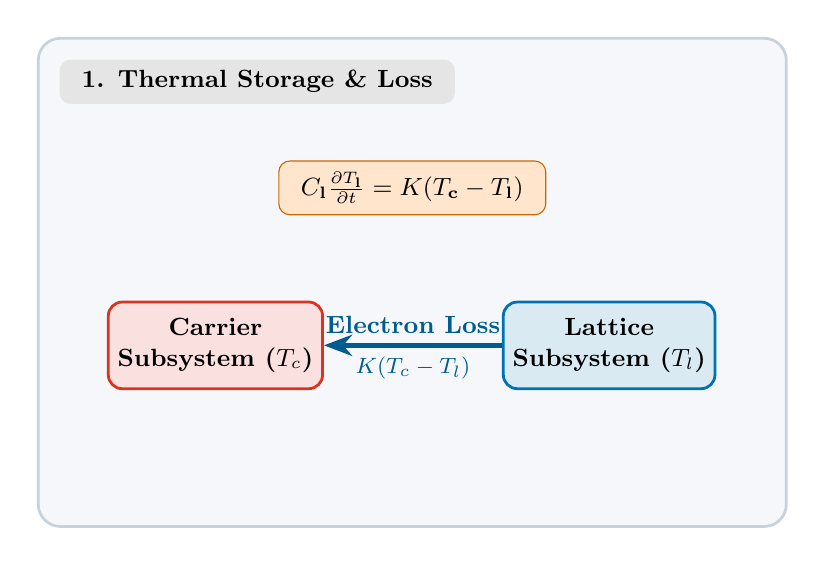
\begin{tikzpicture}[
    >=Stealth,
    font=\sffamily,
    panel/.style={
        fill=panelbg,
        draw=panelborder,
        line width=1pt,
        rounded corners=8pt,
        inner sep=10pt,
        minimum width=9.5cm,
        minimum height=6.2cm,
        align=center
    },
    titlebox/.style={
        draw=none,
        fill=gray!20,
        rounded corners=4pt,
        font=\bfseries\small,
        inner xsep=8pt,
        inner ysep=4pt
    },
    subbox/.style={
        draw,
        rectangle,
        rounded corners=5pt,
        minimum width=2.4cm,
        minimum height=1.1cm,
        align=center,
        font=\small\bfseries,
        line width=1pt
    }
]

    \matrix (m) [matrix of nodes, nodes in empty cells] {
        \node[panel] (p1) {}; \\
    };

    % -------------------------------------------------------------------------
    % PANEL 1: THERMAL STORAGE & LOSS
    % -------------------------------------------------------------------------
    \node[titlebox, anchor=north west] at (p1.north west) [xshift=8pt, yshift=-8pt] {1. Thermal Storage \& Loss};
    \node[titlebox, fill=orange!20, draw=orange!80!black] (p1_eq) at ([yshift=1.2cm]p1.center) {
        $C_{\text{l}}\frac{\partial T_{\text{l}}}{\partial t} = K(T_{\text{c}} - T_{\text{l}})$
    };
    \node[subbox, fill=carrierred!15, draw=carrierred] (carrier_box) at ([xshift=-2.5cm, yshift=-0.8cm]p1.center) {
        Carrier\\Subsystem ($T_c$)
    };
    \node[subbox, fill=latticeblue!15, draw=latticeblue] (lattice_box) at ([xshift=2.5cm, yshift=-0.8cm]p1.center) {
        Lattice\\Subsystem ($T_l$)
    };
    \draw[->, line width=1.6pt, latticeblue!80!black] (lattice_box) -- (carrier_box)
        node[midway, above, font=\small\bfseries] {Electron Loss}
        node[midway, below, font=\footnotesize] {$K(T_c - T_l)$};

\end{tikzpicture}
\end{document}
